\section{Kommunikationskostenoptimierung}
\hyphenation{High--Per-for-mance}
\hyphenation{Per-for-mance}
\hyphenation{Com-pu-ting}
\hyphenation{Be-rech-nungs-eng-pass}
Das Papier \cite[Kap.3]{mainpaper} beschreibt in seinem dritten Kapitel Strategien zur Reduktion von Kommunikationskosten bei der Umsetzung der 3D-FFT in einer High-Performance Architektur.\\

Die Kommunikation findet im High-Performance Kontext zwischen verschiedenen Prozessen/Prozessoren statt, deren lokale Daten aktualisiert werden m"ussen.\\
Kommunikationskosten sind dabei die verwendeten Aufw"ande in Zeit f"ur Synchronisationsabschnitte zwischen einzelnen Datenverarbeitungsschritten.\\

Durch die Ergebnisse aus dem vorigen Kapitel, in dem verschiedene M"oglichkeiten zur Umsetzung der 3D-FFT auf Grafikprozessoren behandelt werden, wird hier die genauere Betrachtung der Kommunikationskostenoptimierung motiviert.\\

Die durch die Verwendung von GPU's erreichte Beschleunigung durch Parallelismus optimiert alle Programmanteile um ein vielfaches mit der Ausnahme der Kommunikation.\\

\begin{figure}
\centering
  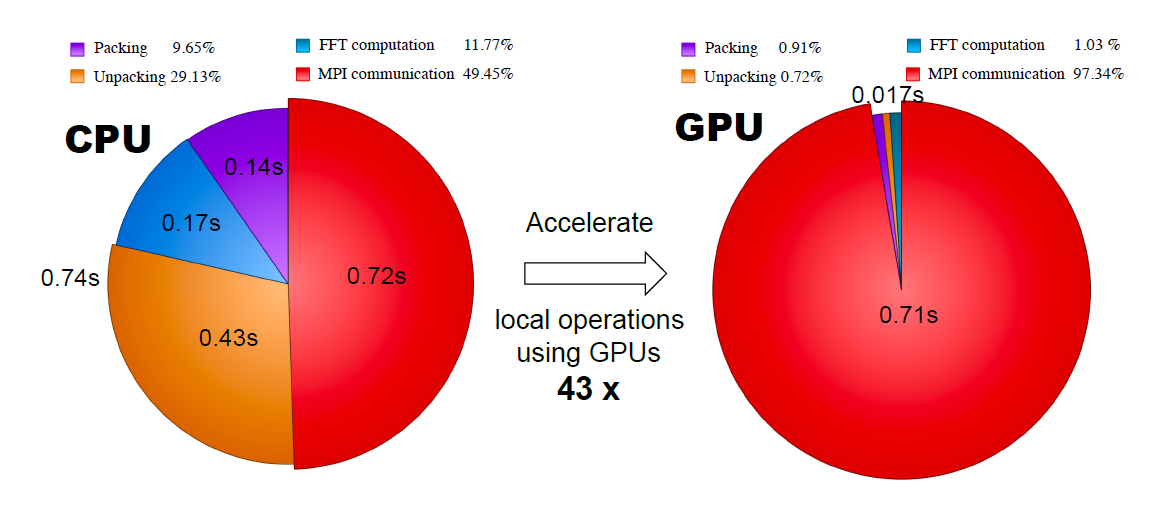
\includegraphics[width=\linewidth]{res/speedup.png}
  \caption{\cite[Abb. 3]{mainpaper} Kreisdiagramme zur Visualisierung von Erfolgen und Bottlenecks bei der GPU Beschleunigung von 3D-FFT's}
  \label{fig:speedup}
\end{figure}

Wie Abbildung \ref{fig:speedup} zeigt hat sich die Zeit, welche im FFT-Algorithmus f"ur Kommunikation zwischen den GPU's/CPU's aufgewendet wird, nur vernachl"assigbar ver"andert. Alle anderen Aktionen (Unpacking, Processing, Packing) haben sich erheblich durch Parallelisierung mit GPUs beschleunigt ($ \frac{0.74s}{0.017s} \approx 43.5$-fache Beschleunigung).\\
\\
Wird Kommunikationszeit mitbetrachtet ist die Beschleunigung $\frac{0.14s+0.17s+0.42s+0.72s}{0.017s+0.71s}=200,8\%$, also nur 2-fach.

Prinzipiell ist Kommunikation ebenfalls parallelisierbar. Da Kommunikation jedoch der Verbreitung einer frisch errechneten, neuen Wahrheit auf anderen Prozessoren dient, h"angt der Grad der Parallelisierbarkeit direkt an der unmittelbaren Wichtigkeit dieser Wahrheit f"ur weitere Berechnungsschritte.\\
Diese Eigenschaft macht Kommunikation hinsichtlich der beteiligten Prozesse oft zu einem inherent seriellen, d.h. in einem gewissen Grad nicht parallelisierbaren Problemanteil.\\
Inherente serielle Anteile in einer Problemstellung limitieren den m"oglichen maximalen Speedup durch Parallelisierung der gesamten Applikation.\\
Diese Sachverhalte k"onnen am FFT-Problem durch die Einteilung in Phasen beobachtet werden. Zwischen jeder Berechnungsphase m"ussen die verwendeten 3D-Tensoren transponiert werden, wodurch neue Werte bei der Werteaufteilung in den Zust"andigkeitsbereich anderer Prozesse fallen und m"ussen daher an diese kommuniziert werden, um die Berechnung fortzuf"uhren.\\
%TODO cite sources
Da Kommunikation unter dem vorgesetzten Ziel der Multi-Prozessorbeschleunigung der Applikation FFT unvermeidbar ist und die Kommunikation selbst zum Berechnungsengpass f"uhrt, muss weiter die Optimierung dieser Kommunikation behandelt werden.


\subsection{Summit Superkomputer}
Für Betrachtungen hinsichtlich Kommunikationsfähigkeit sind Kenntnisse über die verwendeten Systeme von Nutzen.\\
Für Umsetzungen und Benchmarking-Test der beschleunigten GPU wurde der Summit Supercomputers des Oak Ridge National Laboratories(ORNL) verwendet, zu dem sich alle Überlegungen in \cite{mainpaper} zu relativieren scheinen.

Der Summit-Supercomputer im Oak Ridge National Laboratory, Tennessee, ist ein Multi-Prozessor-Supercomputer, der seit 2018 in Betrieb ist. Der Verwendungszweck des Rechners ist der Einsatz in der Wissenschaft.

\subsubsection{Komponenten}

\begin{figure}
\centering
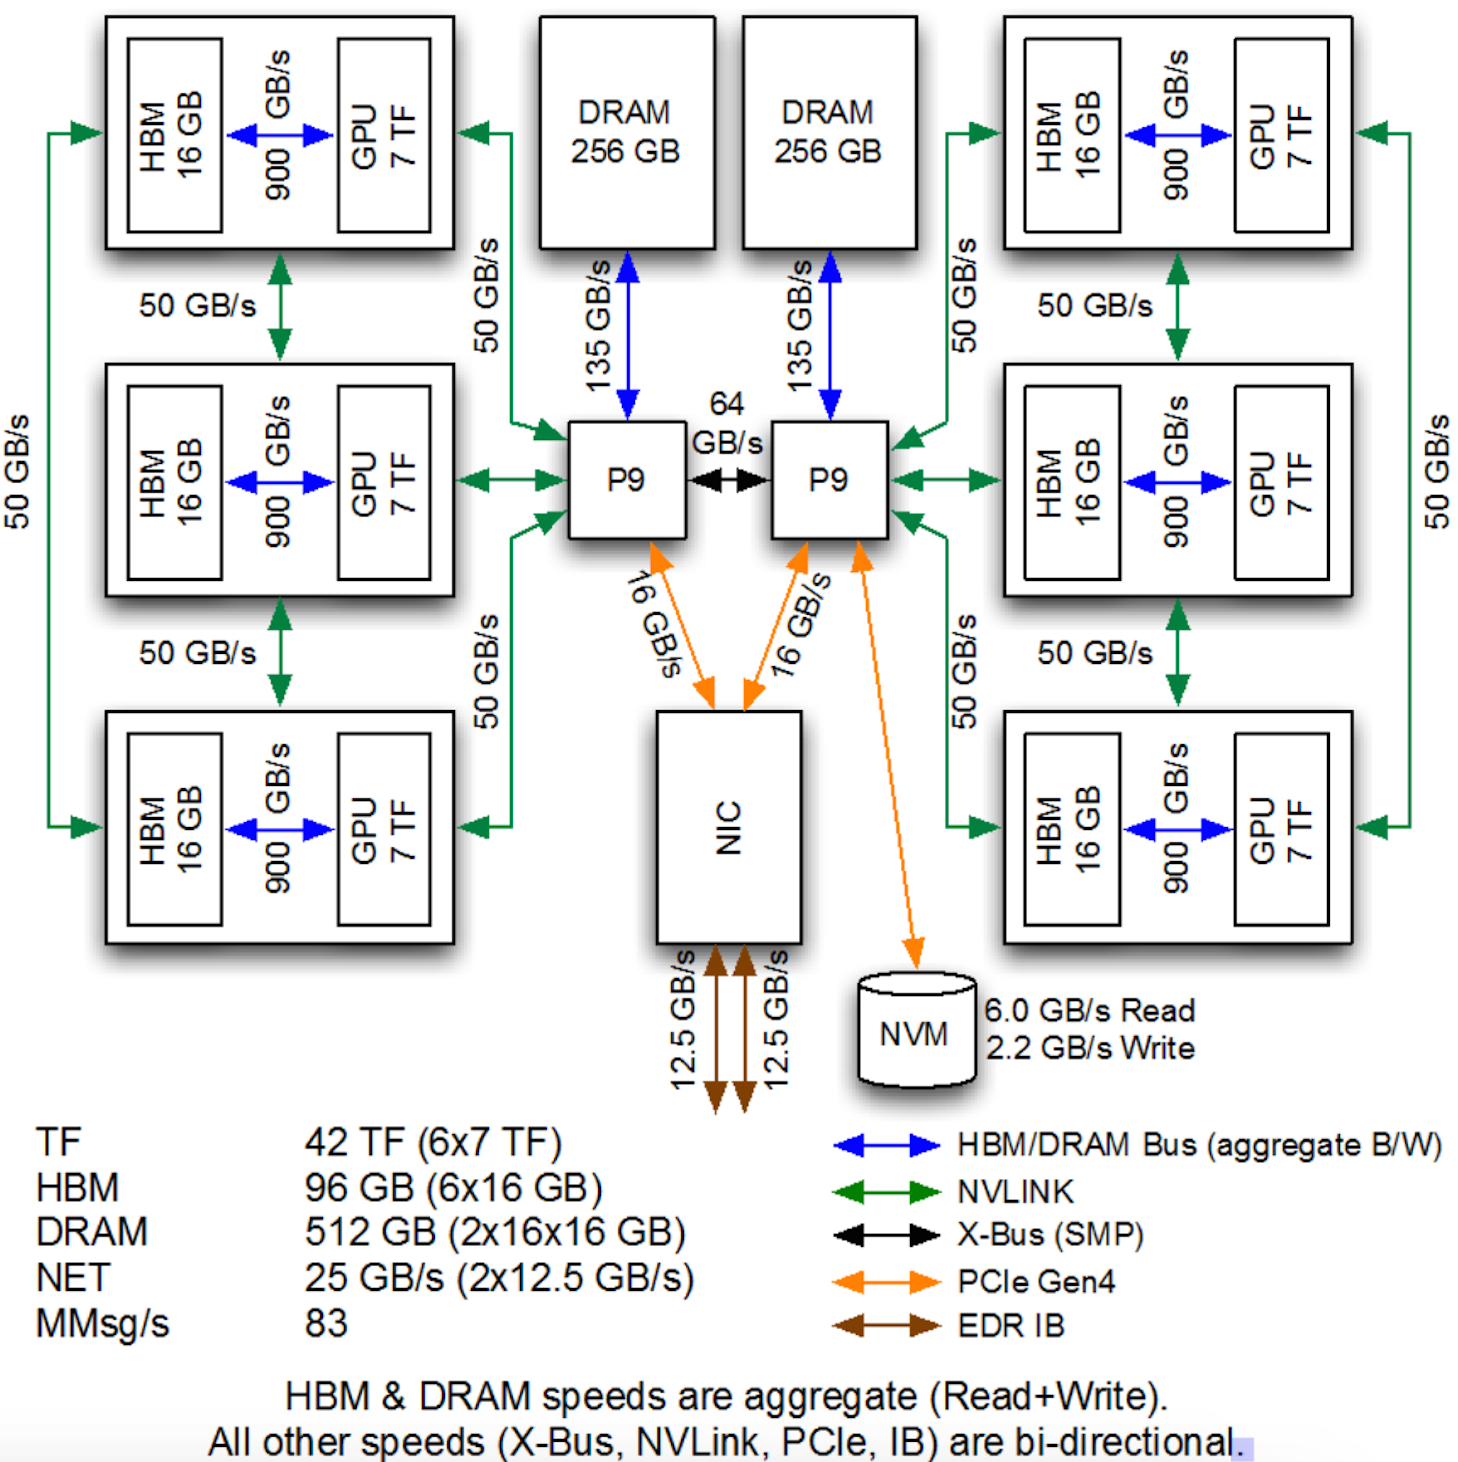
\includegraphics[width=0.6\textwidth]{res/architecture.png}
\caption{\cite[Abb. 1]{mainpaper} Aufbau eines Knotens des Summit Supercomputers, verwendete Kommunikationstechnologien und Komponenten}
	\label{fig:architecture}
\end{figure}
\begin{enumerate}
	\item 4608 Knoten gesamt
	\item je 2 CPU's (IBM POWER9, in der Graphik unter P9)
	\item je 6 GPU's (NVIDIA Volta V100s)
\end{enumerate} \cite{osummit}
Abbildung \ref{fig:architecture} zeigt die generelle Systemarchitektur eines Knotens des Summit rechners.\\
Eine CPU und 3 GPU's sind unter einem CPU-Sockel zusammengefasst. Es befinden sich 2 solcher Sockel auf einem Summit-Knoten. Zwischen allen Prozessoren unter einem Sockel existieren P2P Verbindungen mit der NVINK Verbindungstechnologie.\\
Die Komponenten können als Stufen von Recheneinheiten angesehen werden:
\begin{enumerate}
	\item Knoten
	\item Sockel
	\item Prozessor
\end{enumerate}

Terminologie zur Unterscheidung von Kommunikationsformen zwischen Sockeln wird wie folgt definiert:\\
\begin{defi}[Same-Socket-Kommunikation (eng. \textit{same-socket-communication})].
Kommunikationsvorg"ange, welche zwischen Prozessoren unter dem selben Sockel erfolgen.
\end{defi}
\begin{defi}[Cross-Socket-Kommunikation (eng. \textit{cross-socket-communication})]
Kommunikationsvorg"ange, welche zwische Prozessoren auf unterschiedlichen Sockeln erfolgen.
\end{defi}
Zur Cross-Socket-Kommunikation auf einem Knoten exisitiert ein X-Bus (64GB/s), der zwischen den CPU's angelegt ist.\\
Theoretisch k"onnen also maximal $\frac{64GB/s}{50GB/s} = 1.28$ Prozessoren cross-socket kommunizerien.\\
Unter der Annahme, dass jeder Prozessor im Schnitt mit jedem anderen Prozess gleich viel kommuniziert  entstehen demnach Kommunikationsengp"asse zuerst bei der cross-socket Kommunikation.\\

\subsubsection{Topologie}
Die Knoten sind untereinander unter einer bestimmten Topologie verbunden. Am Summit-Rechner wurde die Fat-Tree Topologie verwendet.\\
\begin{figure}
\centering
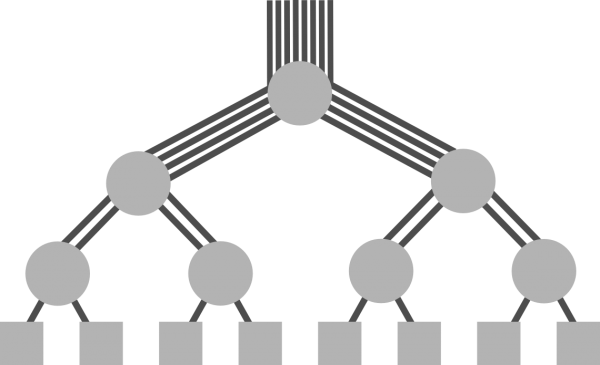
\includegraphics[width=0.4\textwidth]{res/fat_tree.png}
\caption{\cite{fattree} Graphische Darstellung der Fat-Tree Topologie}
	\label{fig:fat_tree}
\end{figure}
Man vergleiche im Folgendes mit Abbildung \ref{fig:fat_tree}
Ein Fat-Tree ist eine Topologie, bei der Switches zu einem Bin"arbaum verkn"upft werden. Endknoten, also Summit-Knoten, werden dabei an den Bl"attern des Baumes platziert.\\
Ma"sgeblich f"ur den Fat-Tree ist dabei die Regel, dass f"ur jeden Switch im System die Anzahl der Verbindungen nach unten gleich der Anzahl der Verbindungen nach oben ist, also für jeden Knoten gleich viel Bandbreite zu den Eltern wie zu der Gruppe aller Kinder verfügbar ist. Daraus folgt die Anzahl der Verbindungen pro switch in Abh"angigkeit der Baumh"ohe $h$, maximaler Baumh"ohe $h_{max}$, Der H"ohe am Wurzelknoten $h_{root}=0$ und der Anzahl der Elternverbindung eines Blattknotens $c$ (hier: $c=1$):
\begin{itemize}
	\item Anzahl Elterverbindungen/Kindverbindungen : $(h_{max}+1-h)*c$
	\item Anzahl Verbindungen pro Kind : $\frac{(h_{max}+1-h)*c}{2}$ bei 2 Kindern
\end{itemize}
Die Verbindungsanzahl ist daher maximal am Wurzelknoten mit $h_{max}+1$, der Baum wird zur Wurzel hin \glqq dicker (eng. \textit{fat})\grqq.\\
H"alt eine Fat-Tree Topologie das Verh"altnis von Eltern- zu Kindverbindung von $1:1$ ein, nennt man diese Non-Blocking. Die Gegenteilige Blocking-Eigenschaft ist bei Nichteinhaltung festzustellen.\\
Ist das Verh"altnis unausgeglichen ist die Kommunikation durch den konkreten unausgeglichenen Switch limitiert. Zum Beispiel k"onnten doppelt so viele Kindverbindungen existieren als Elternverbindungen ($1:2)$. So k"onnen verh"altnism"a"sig viele Kindknoten "uber den Switch zeitgleich kommunizieren, jedoch kann nur die H"alfte aller Kindkommunikation an Eltern weitergereicht werden. Man spricht bei diesem Beispiel von einem Blocking-Faktor von 2, Kind zu Eltern.\\
\\
Die Topologie erreicht durch die das exponentielle Wachstum des Bin"arbaumes mit der Baumtiefe leicht eine gro"se Anzahl verkn"upfbarer Prozessoren ($2^h_{max}$). (vgl. \cite{fattree})\\
\\


\subsection{Relevante Technologien}
\cite{mainpaper} benennt einige verwendete Technologien, gibt jedoch selbst dem Leser oft wenig Kontext zu diesen. Deshalb wird im Folgenden zu diesen Technologien der Kontext hergestellt.

\subsubsection{ NVLink }
Eine proprietäre Verbindungstechnologie auf Prozessorebene, entwickelt von NVIDIA.\\
Traditionell kommunizierten Prozessoren in einer Systemarchitektur ausschlie"slich über den PCIe-Bus. NVLink erlaubt zusätzliche P2P Verbindungen zwischen Prozessoren und erhöht daduch massiv die kommunikativen Eigenschaften der gesamten Systemarchitektur (vgl. \cite{nvlink}).\\
Die Technologie ist besonders für die Verarbeitung von großen Datenmengen in z.B. Datenzentren wertvoll.\\
\\
Unidirektional bietet die Technologie bei den verwendete Prozessoren 25GB/s. Die Technologie ist allerdings konzeptionell bidirektional, wodurch die in Abbildung \ref{fig:architecture}, d.h. \cite[Abb. 1]{mainpaper} 50GB/s zu Stande kommen.\\
\cite[FAQ, What is NVLink?]{osummit} gibt allerdings an, dass zwischen 2 Prozessoren auf einem Sockel im Summit Supercomputer 2 NVLink-Verbindungen angelegt sind, was die bandbreite theoretisch auf 100GB/s anhebt.

\subsubsection{ NVIDIA GPUDirect }
NVIDIA GPUDirect ist eine Technologie, die den direkten Zugriff von P"aripherie auf den Speicher von NVIDIA GPU's zul"asst. Dieser Vorgang wird als \textit{Remote Direct Memory Access (RDMA)} bezeichnet.\\
Dadurch wird der traditionelle Umweg "uber RAM vermieden. Beispiele f"ur P"aripherien sind Netzwerkadapter, Speicher (wie Solid State Drives) und andere Graphikkarten (vgl. \cite{gpud}).\\
Vor allem Letztere sind im Kontext dieses Papiers von Bedeutung.

\subsubsection{ \textit{Message Passing Interface} (MPI) }
MPI ist ein Standard, der Schnittstellen f"ur den Nachrichtenaustausch zwischen Prozessen spezifiziert.\\
Portabilit"at und Einfachheit werden als prim"are Ziele angegeben (vgl. \cite[Kap. 1.1]{mpi}).\\
Es gibt mehrere Implementierungen dieses Standards, zum Beispiel die Open-Source-Variante OpenMPI (\cite{openmpi}).\\
In verteilten Systemen wird MPI als Abstraktion f"ur die Kommunikation zwischen parallelen Prozessoren/Prozessen verwendet.

\subsubsection{ CUDA }
Die \textit{\textbf{C}ompute \textbf{U}nified \textbf{D}evice \textbf{A}rchitecture (CUDA)}, entwickelt von NVIDIA ist eine Plattform und Programmiermodell f"ur parallele Berechnungen auf NVIDIA GPUs (vgl. \cite{cuda}v).\\
Die Technologie gewährt niedrigabstrakten Zugriff auf Rechenressourcen von NVIDIA Grafikprozessoren und ermöglicht so performante Implementierungen.

\subsubsection{ CUDA-aware MPI }
Ist eine Kombination aus CUDA und MPI.\\
Da CUDA mit dem MPI Standard kompatibel ist, sind MPI-Implementierungen durch CUDA m"oglich. Die resultierende MPI-Implementierung ist niedrigabstakt und plattformspezifischer und soll dadurch in vielen F"allen eine bessere, performantere Umsetzung des MPI-Standards im Speziellen auf NVIDIA GPUs darstellen.

\subsection{Weitere Spezielle Terminologie}

\subsubsection{MPI\_Alltoall}
\textit{MPI\_Alltoall} ist eine Kommunikationsroutine des Message Passing Interfaces. Dabei Senden alle $N$ Prozesse Nachrichten der selben Gr"o"se zu allen $N$ Prozessen (inklusive dem eigenen Prozess). Der Kommunikationsaufwand betr"agt also $N^2 * Nachrichtenl"ange$.\\
Es wird ein Kommunikationspuffer verwendet, dessen Gr"o"se $N*Nachrichtenl"ange$ betr"agt. (vgl. \cite{MPImanpage})\\
Im Papier \cite{mainpaper} scheint eine spezielle Implementierung von MPI\_All2All f"ur den Summit Computer verwendet.

\subsubsection{MPI P2P}
Als Peer to Peer (P2P) Kommunikation bezeichnet man eine Kommunikationsstrategie, bei der alle n"otigen Informationen von einem kommunizierenden Knoten zum anderen direkt und nach Bedarf ausgetauscht werden. 
Dabei sind die Parameter der konkreten Kommunikation prinzipiell an keine weiteren Eigenschaften gebunden.\\
\cite{mainpaper} scheint nicht genau auf die Realisierung dieser Strategie einzugehen. Da der MPI-Standard keine P2P funktion zu definieren scheint, kann an dieser Stelle angenommen werden, dass diese Art der Kommunikation durch MPI\_Send und MPI\_Recv aufrufen realisiert wird, welche als die nativen Sendebefehle in MPI zu verstehen sind.\\
Auch hier scheint das Papier \cite{mainpaper} wieder eine spziielle Implementierung f"ur den Summit Computer zu referenzieren.

\subsubsection{Kommunikationsrichtung}
\begin{defi}[Unidirektionale Kommunikation (\textit{ eng. unidirectional communication })]
In einem abgeschlossenen Kommunikationsvorgang zwischen $p1$ und $p2$ werden Daten ausschlie"sslich von $p1$ nach $p2$ kommuniziert.
\end{defi}
\begin{defi}[Bidirektionale Kommunikation (\textit{ eng. bidirectional communication })]
In einem abgeschlossenen Kommunikationsvorgang zwischen $p1$ und $p2$ k"onnen Daten sowohl von $p1$ nach $p2$, als auch von $p2$ nach $p1$ gleichzeitig ausgetauscht werden.
\end{defi}

\subsubsection{3D-FFT Datenkomposition}
Der Input der 3D-FFT ist ein 3D-Tensor. Die daraufhin ben"otigten Operationen zu Berechnung der FFT sind abh"angig vom Algorithmus. Jedoch k"onnen durch eine effiziente B"undelung von von einer Operation gemeinsam ben"otigten Information Kommunikationskosten gespart werden.
\cite{mainpaper} verwendet daher folgende Datenkompositionen:
\begin{enumerate}
	\item \textit{pencil}\\
		Zu Deutsch Stift, suggeriert einen eindimensional ausgedehnten Anteil am Tensor, also ein 3D Tensor mit einer der Dimensionen $\{1,1,N\},\{1,N,1\},\{N,1,1\}$.
	\item \textit{slab}\\
		Zu Deutsch Platte, suggeriert einen zweidimension ausgedehnten Anteil am Tensor, also ein 3D Tensor mit einer der Dimensionen $\{N,N,1\},\{N,1,N\},\{1,N,N\}$.
\end{enumerate}

\subsection{L"osungsans"atze}
Konzeptionell gibt es 2 Optionen um Kommunikationskosten zu verringern.
\begin{itemize}
	\item Option1: Verwendung eines besseren Algorithmus hinsichtlich serieller Anteile und Kommunikation.
	\item Option2: Verbesserung der Kommunikationsstrategie unter Einbeziehung von Eigenschaften der Systemarchitektur.
\end{itemize}

\subsubsection{Ansatz 0}
Benchmarks zur Ermittlung tatsächlicher Bandbreiten (hinführend zu Option 2).
\begin{figure}
\centering
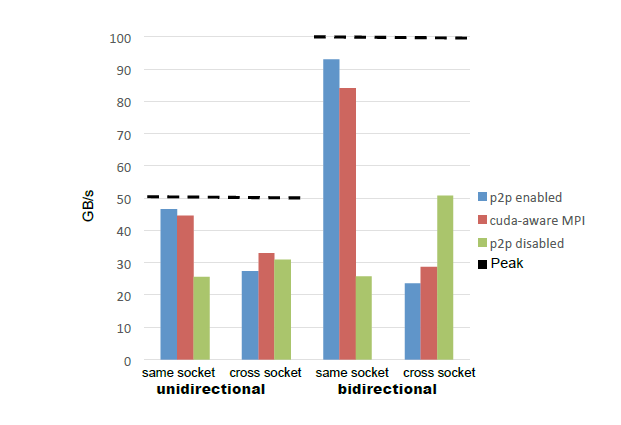
\includegraphics[width=0.6\textwidth]{res/bench0.png}
\caption{\cite[Abb. 4]{mainpaper} Benchmark der Bandbreite für verschiedenene Möglichkeiten der P2P Kommunikation}
	\label{fig:bench0}
\end{figure}
Untersuchungen sind
\begin{itemize}
	\item same socket vs. cross socket
	\item unidirectional vs. bidirectional
	\item p2p vs. cuda-aware MPI vs. p2p deaktiviert
\end{itemize}
Ergebnisse sind in Abbildung \ref{fig:bench0} zu betrachten.\\
Am meisten Druchsatz wurde same-socket, bidirectional über non-cuda p2p erreicht, dicht gefolgt von der cuda-aware Variante.\\
Das Ergebnis macht theoretisch Sinn: Die zwischen den same-socket Prozessoren verwendete NVLink Verbindungstechnologie erlaubt verlustfrei bidirektionale Datenübertragung. Der theoretische Effekt von insgesamt doppelter Bandbreite ist in Abbildung \ref{fig:bench0} deutlich sichtbar.\\


\subsubsection{Ansatz 1}
\begin{figure*}
	\begin{subfigure}[t]{0.5\textwidth}
		\centering
		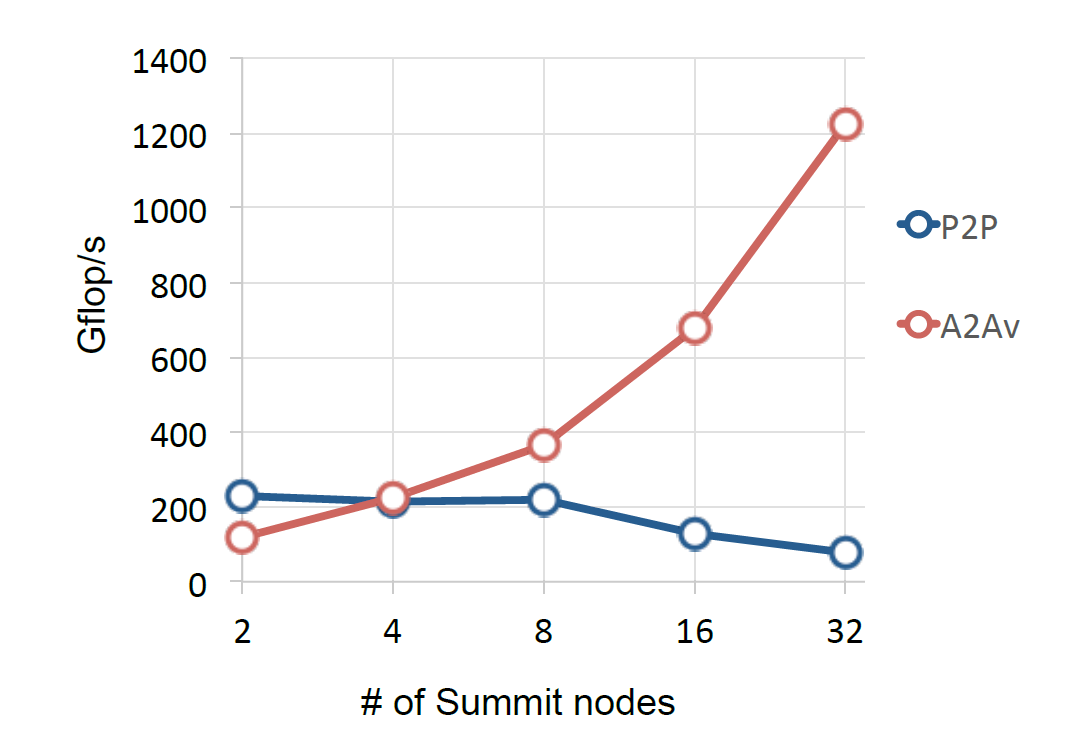
\includegraphics[width=1\textwidth]{res/bench.png}
		\caption{\cite[Abb. 5]{mainpaper} Benchmark P2P vs A2A Gflops/s \& Anzahl Knoten}
		\label{fig:bench}
	\end{subfigure}
~
	\begin{subfigure}[t]{0.5\textwidth}
		\centering
		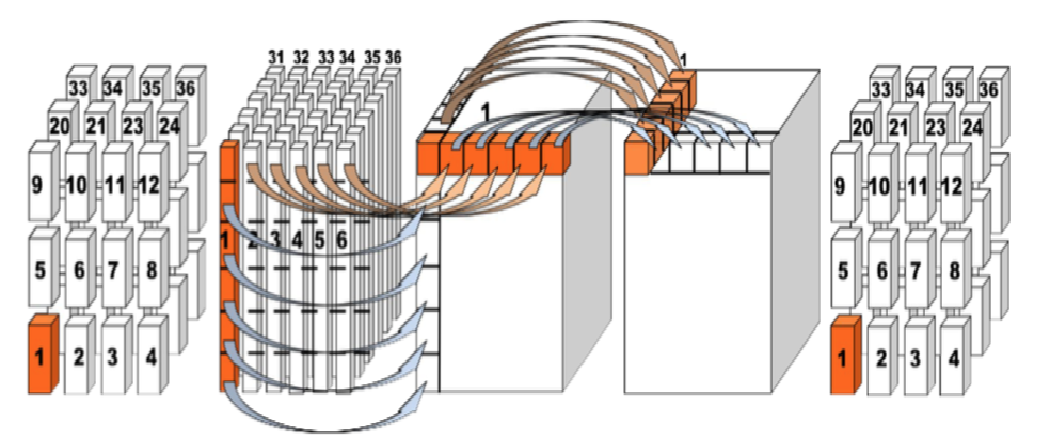
\includegraphics[width=1\textwidth]{res/algo.png}
		\caption{\cite[Abb. 2]{mainpaper} Prinzipieller Aufbau des 3D-FFT Algorithmus. }
		\label{fig:algo}
	\end{subfigure}
	\caption{Zwei begleitende Abbildungen zu Lösungsansätzen 1 und 2}
\end{figure*}


Abbildung \ref{fig:bench} zeigt das Ergebnis eines Benchmarking-Versuchs mit dem Verh"altnis von Prozessor-Operationen (in Gflops/s) zu der Anzahl der verwendeten Summit-Knoten.\\
Verwendete Strategien sind:
\begin{enumerate}
	\item Summit MPI Alltoall
	\item Summit MPI P2P
\end{enumerate}
Die Unterschiede sind nicht Algorithmisch. Die Untersuchung bezieht sich also auf die kommunikativen Eigenschaften der Systemarchitektur (Option 2).\\
Ergebnis: Stategie 2 scheint f"ur geringer als 4 Knotenzahlen besser zu sein, sinkt jedoch sogar nacher weiter ab.
Strategie 1 scheint generell jedoch besser zu skalieren und "ubernimmt bei mehr Knoten stark die F"uhrung.\\
\cite{mainpaper} geht jedoch selbst weiter nicht auf eine m"ogliche Begr"undung ein.\\
Bei diesem Lösungsansatz wurde die Superiorität von All2All in Punkten Zeit und Skalierbarkeit festgestellt.\\
Dieses Ergebnis ist theoretisch Sinnvoll, da, wie die Abbildung \ref{fig:algo} zeigt, All2All Kommunikation die Bedürfnisse der 3D-FFT Applikation nahezu exakt abbildet.\\
Sei ein \textit{Pencil} der Länge $N$ gegeben, so erzeugt ein Prozess $N$ Werte für $N$ Folgeprozesse. Auf den Folgeprozessen wird aus den Teilergebnissen (einzelne Werte) ein neuer \textit{Pencil} der Länge $N$ zusammengefügt.\\
In All2All Kommunikation wird ein Buffer der Länge $N$ angelegt. Dieser Buffer wird durch die 1D-FFT Operation befüllt. Die einzelnen Werte werden durch All2All an die Folgeprozesse verteilt.

\subsubsection{Ansatz 2}
Die Kommunikation kann algorithmisch ge"andert werden (Option 1).\\
Der zuerst vorgestellte Algorithmus agiert in den Phasen:
\begin{enumerate}
	\item Transform X
	\item Transform Y
	\item Transform Z
	\item Move Back to Original
\end{enumerate}
(vgl. Abbildung \ref{fig:algo})\\
Zwischen den Phasen wird kommuniziert. Die Kommunikation verh"alt sich zu den jeweiligen Phasen sequenziel, d.h. ist nicht mit einer Phase parallelisierbar, oder f"ahig zu Pipelining.\\
K"onnen die kommunikativen Anteile der Phasen zusammengefasst werden ergibt sich daraus weniger redundante, serielle Kommunikation.\\
Hier wird dies in Form von \textit{Slab}-Datenkomposition durchgef"uhrt.
Zuvor erhielten Prozesse eine Dimension des 3D-FFT-Input Datentensors, auf dem eine 1D-FFT berechnet wird. Dann werden die Ergebnisse propagiert und dabei der Tensor Transformiert.\\
F"ur diesen Ansatz erhalten Prozesse jedoch 2 Dimensionen des 3D-FFT-Input Datentensors. Demnach kann der Prozess beispielsweise folgenderma"sen abgehandelt werden:
\begin{itemize}
	\item[1.1] Berechne 1D-FFT auf allen Zeilen im bekannten 2D-Tensor. Die Ergebnisse sind implizit als neuer 2D Tensor zusammengef"ugt.
	\item[1.2] Berechne FFT's f"ur alle Spalten im Ergebnistensor.
	\item[2.0] Transform Z
	\item[3.0] Move Back to Original.
\end{itemize}
Man beachte, dass Schritt 1.1 und 1.2 ohne Kommunikation auskommen, da alle ben"otigten Informationen in \textit{Slab}-Datenkomposition aus Schritt~1.1~in Schritt 1.2 bekannt sind.\\
Es werden weniger Informationen redundant zwischen Phasen ausgetauscht (\textit{Pencil} 4 Phasen, \textit{Slab} 3 Phasen).\\
Ein Prozess kann also 2 Phasen der FFT Berechnung ohne Kommunikation durchf"uhren.\\
Theoretisch wurden demnach 25\% Kommunikationskosten eingespart.\\
\\
Ein Problem dabei, auf den \cite{mainpaper} nicht eingeht, ist der quadratisch erh"ohte Speicherverbrauch pro Knoten, so wie der quadratisch erh"ohte Kommunikationsaufwand in der ersten Kommunikationsphase.\\
K"onnen die Knoten diese quadratische Speicherlast tragen ist dieser Ansatz jedoch eine solide Option. Die quadratische Kommunikation scheint sich ebenfalls nicht in den sp"ater angebenen Werten f"ur die erreichten Speedups durch die Durchf"uhrung dieses Ansatzes widerzuspiegeln.

\subsubsection{Ansatz 3}
Vor der Ausführung des Algorithmus werden dynamische Analysen für erwartete Lasten bei der Ausf"uhrung durchgeführt. Dadurch können Berechnungsressourcen je nach Problemgröße hinsichtlich der Kommunikation optimal gewählt werden (Option 2).\\
Man versucht dabei allokierte Ressourcen möglichst maximal auszulasten, um Kommunikation so gut wie möglich komplett zu vermeiden.\\
Der Ansatz ist übertragbar auf die verschiedenen Stufen von Komponenten in der Systemarchitektur:
\begin{enumerate}
	\item Knoten
	\item Sockel
	\item Prozessor
\end{enumerate}


